\documentclass[11pt, letterpaper]{article}

\usepackage[left=3cm, right=3cm, top=1in, bottom=1in]{geometry}
\usepackage[spanish, es-noshorthands]{babel}
\usepackage[style=ieee]{biblatex}

\usepackage{hyperref}
\usepackage{mathptmx}
\usepackage{graphicx}
\usepackage{svg}
\usepackage{csquotes}
\usepackage{dirtytalk}
\usepackage[most]{tcolorbox}
\usepackage[shortlabels]{enumitem}
\usepackage{lipsum}
\usepackage{pgfgantt}
%% CONFIGURACIONES DEL PROYECTO

\addbibresource{./main.bib}

\newtheorem{definition}{Definición}

\newlist{syllabus}{enumerate}{10}
\setlist[syllabus]{label*=\arabic*., font=\bfseries, leftmargin=*}
\setlistdepth{10} 

\def\student{Ernesto Carlos Arena Alarcon}
\def\tutor{Jorge Antonio Nava Amador}
\def\professor{Jorge León}
\def\college{Universidad Mayor de San Andrés}
\def\collegefaculty{Facultad de Ingeniería}
\def\collegefield{Ingeniería Electrónica}
\def\collegelogo{assets/umsa.png}
\def\documenttitle{Perfil de Proyecto de Grado}
\def\projecttitle{ERFACTO: Sistema MRP (Material Resource Planning) para la empresa de prefabricados ArenA}
%% ESTRUCTURA DEL DOCUMENTO

\begin{document}
\begin{titlepage}
    \centering
    {\bfseries \large \college - \collegefaculty \par \collegefield }\\[2cm]

    \includegraphics[width=0.2\textwidth]{assets/umsa.png}
    \\[1cm]

    {\LARGE \MakeUppercase{\documenttitle}}\\[1cm]

    \textbf{\Large \MakeUppercase{\projecttitle}}
    \vfill
    \MakeUppercase{Postulante: } \MakeUppercase{\student}\\[1cm]

    \MakeUppercase{Asesor: } \MakeUppercase{\tutor}\\[1cm]

    \MakeUppercase{Docente D.A.M.: } \MakeUppercase{\professor}\\[1cm]

    \vfill
    {La Paz, \today\par}
\end{titlepage}
%%\begin{abstract}
\end{abstract}
\tableofcontents
\newpage
% \input{./section/introduction}
% \section{Antecedentes}

Durante el desarrollo del sistema SIAI (Sistema de Información Ambiental Industrial) del \say{Ministerio de Desarrollo Productivo y Economía Plural} por parte de la empresa \say{2IES},
se pudo identificar ciertas funcionalidades comunes a muchos sistemas de software gubernamentales,
las cuales tienen que ver con los trámites, un proceso común en la administración pública de los gobiernos.

% MARK: Estado
\subsection{El Estado como Sistema Organizativo}

% Por qué hablaremos del estado
Si bien los temas filosóficos, históricos o políticos parecen carecer de importancia en la presente propuesta,
es importante entender el origen de la problemática señalada más adelante a partir de la concepción misma del gobierno y del estado, pues esto nos encaminará a entender su evolución organizativa,
la cual eventualmente da lugar a la cuestión que se trata en este documento.

% Origen del estado
Para explicar el origen de la organización social y su evolución, que derivará posteriormente en la creación del estado, se pueden identificar dos grandes teorías:
Teoría de la armonía social y teoría del conflicto \cite{vacarofernandezOrigenEstado2000}.
La primera propone que la sociedad se organiza a sí misma como una expresión de solidaridad basada en una conciencia común,
mientras que la segunda indica que lo hace por una tendencia a resolver contradicciones y tensiones.
Para los teóricos de la armonía social, \textquote{el estado aparece como la solución colectiva de necesidades nuevas que surgen a partir de situaciones también nuevas}\cite[3]{vacarofernandezOrigenEstado2000}.

% Definición básica del estado
Para lo que nos atañe, el estado es un fenómeno político que supuso la separación o la salida de lo político del terreno social y
\textbf{la conversión del individuo en un ciudadano}, cuya relación de pertenencia fundamental será con el estado al margen de cualquier característica particular \cite{gordilloperezPorQueSurge2017}.
Esto implica que el ciudadano tiene en adelante una serie de obligaciones para con el estado al cual pertenece, así como derechos.

% Listado de los componentes del estado
El estado no podría terminar de definirse sin mencionar los componentes o elementos que lo acaban materializando, que son 4 \cite{delarocharadaElementosParaTeoria2019}:

\begin{itemize}
    \item Territorio
    \item Población
    \item Gobierno
    \item Soberanía
\end{itemize}

% MARK: Gobierno
\subsection{Gobierno, Burocracia y Administración Pública}

Dentro de los 4 componentes listados, el gobierno
(del griego $\kappa \upsilon \beta \varepsilon \rho \nu \acute{\epsilon} \iota \nu$ kybernéin \textquote{pilotar un barco} o \textquote{capitán de un barco}),
es un sistema orgánico de autoridades a través del cual se expresa el poder del Estado, creando, afirmando y desenvolviendo el orden jurídico \cite{fernandezruizDerechoParlamentario2023}.
Es por tanto un actor que materializa el poder del estado hacia la población.

% Necesidad de practicar la burocracia
Este sistema requiere casi siempre la práctica de la burocracia
(término acuñado en el siglo 18 por el filósofo Francés Vincent de Gournay, derivando del francés \textit{bureau} y \textit{cratie} que significan \say{Escritorio para escribir} y \say{Gobierno} respectivamente \cite{rockmanBureaucracyStructureProcesses2024}),
que según Weber es técnicamente la forma más avanzada de ejercer o empuñar el poder por aquellos que lo controlan \cite[114]{watersWeberRationalismModern2015} (el gobierno).

% Qué es burocracia
El mismo sociólogo alemán, Max Weber, define burocracia como una forma racional de organización que en su opinión es la forma más pura de sistema legal de autoridad.
La burocracia es según él, necesaria y algunas de sus características fundamentales son las jerarquías, la especialización y la definición estricta de reglas y regulaciones \cite{archerDictionaryPublicAdministration2022}.
Increíblemente y, a pesar de la experiencia popular, la burocracia se supone en principio como una manera racional de organizar de forma eficiente.

% Crítica a la burocracia
Sin embargo, esta forma de organización suele tener como consecuencia en la práctica una connotación negativa, %% No sólo una connotación
ya que implica el consumo de mayores tiempos de ejecución para distintas tareas administrativas, como es el caso del trámite.

% Presentación de la administración pública
Este tipo de organización aplicada de forma transversal en las distintas instituciones del gobierno,
convive con otra figura importante y también transversal, que es la de la administración pública,
que es \textquote{la que tiene la gestión de los asuntos comunes respecto al ciudadano como miembro del estado} \cite{guerreroCharlesJeanBonninSiglo2020}.

% Origen de la administración pública
La concepción de administración pública se remonta a muchos años atrás.
Por ejemplo, en el año 302 D.C. Claudio Mamertino ya hablaba del término \say{administración de la cosa pública} (\textit{administratione res publicae}) \cite{nixonPraiseLaterRoman1994}.
Y es que está estrechamente relacionada con el ejercicio de cualquier tipo de gobierno.
Sin embargo, la aplicación y definición de la misma no estaría clara hasta la llegada de \textbf{Charles-Jean Baptiste Bonnin} (1772-1846),
el padre de la ciencia de la administración pública moderna.

% El trámite es un mecanismo de contacto del pueblo con el estado mediante la administración
La administración pública pone en contacto directo a la población con el poder político \cite{mostajomachicadoDerechoAdministrativoAdministracion2016}
y lo hace de forma inmediata a diferencia de algún poder como el legislativo o el judicial, los cuales se contactan con el ciudadano de forma mediata.
Aunque las maneras de efectuar este contacto pueden ser varias, la ciencia de la administración pública no aborda exhaustivamente las mismas.
Sin embargo, desde una perspectiva heurística y basada en la experiencia, como ciudadano de un estado, parece evidente que una de las formas más comunes es aquella que se realiza mediante el trámite.

% MARK: Trámite
\subsection{El trámite}

Poco se ha escrito estrictamente sobre los trámites a nivel académico.
El mismo término parece ser poco universal y tener especial significado en el español de la región.
En inglés, por ejemplo, no existe una traducción exacta para la palabra trámite.
Sin embargo, por conocimiento popular se sabe lo que significa.
Se sabe también lo estrechamente relacionado que está con el gobierno, la burocracia y el manejo de documentos y,
a pesar de que también se puede usar en otros contextos, la sociedad parece asociarlo casi siempre con lo aquí descrito.

La palabra trámite viene del latín \say{\textit{trames}}, \say{\textit{tramitis}}, que para los romanos significaba \say{senda}, \say{camino}, de donde se derivó el sentido actual de \say{vía legal o procedimiento que debe seguir una gestión}\cite{TramiteCastellanoPagina}.
En inglés no existe una palabra que tenga la traducción exacta de trámite, pero en la literatura de este idioma se usan distintas palabras como \say{\textit{Procedure}}, \say{\textit{Transaction}} o \say{\textit{Paperwork}}.
También en español se puede referir al mismo como \say{Procedimiento administrativo} o \say{Servicio Público Transaccional}.
En todas estas definiciones se tiene como común denominador a los términos: Proceso, Camino, Papeleo, Transacción.

% MARK: Trámite Defs.
Al respecto, de acuerdo a una definición que el Gobierno de México indica en uno de sus portales web, se entiende como trámite a:

\begin{displayquote}
    Cualquier solicitud o entrega de información que las personas físicas o morales del sector privado hacen ante una dependencia u organismo descentralizado,
    ya sea para cumplir una obligación, obtener un beneficio o servicio o, en general, a fin de que se emita una resolución, así como cualquier documento que dichas personas estén obligadas a conservar \cite{epnQueEsTramite}.
\end{displayquote}

En el mismo portal se hace una clasificación de los trámites, donde se señalan 5 tipos de los mismos:

\begin{enumerate}
    \item De naturaleza obligatoria
    \item De beneficio
    \item De conservación
    \item De procedimiento
    \item De consulta
\end{enumerate}

Según la Real Academia de la Lengua Española, se define como:
\say{Cada uno de los pasos y diligencias que hay que recorrer en un asunto hasta su conclusión} \parencite{asaleDiccionarioLenguaEspanola}.

Los trámites, también llamados \say{servicios públicos transaccionales}, constituyen además
el conjunto de requisitos, pasos o acciones a través de los cuales los individuos o las empresas piden o entregan información a una entidad pública, con el fin de obtener un derecho o para cumplir con una obligación \cite[36]{rosethFinTramiteEterno2018}.
Desde esta definición, se puede agrupar a los trámites en las siguientes cuatro categorías:

\begin{enumerate}
    \item Registros, certificaciones y constancias
    \item Obligaciones
    \item Servicios
    \item Permisos
\end{enumerate}

% MARK: Trámite Probs.
Sin embargo, el proceso del trámite puede llegar a ser muy engorroso y perjudicar a los ciudadanos.
Tal es el caso de \textbf{Domitila Murillo}, quien a causa de un trámite debía trasladarse entre varias ciudades de Bolivia para hacer largas filas y vagar perdida entre una cantidad indefinida de requisitos.
Cuando finalmente logró recibir su cédula (el motivo del trámite), no le quedaron más que dos semanas antes de fallecer \cite{charoskyQuejaComoEnergia2014}.

El caso de Domitila no es aislado, por supuesto.
Las distancias, la falta de definición en los requerimientos y la burocracia afectan al proceso del trámite.
El tiempo que demandan suele causar un perjuicio para la población, muchas veces llegando a tardar horas por un simple trámite, como se puede ver en la figura \ref{fig:horastramite}.
En esta figura se puede ver que en Bolivia, por ejemplo, un trámite puede durar alrededor de 11 horas. Esto tiene también un impacto económico sobre la gente.

\begin{figure}[htbp]
    \centering
    \includegraphics[width=0.7\textwidth]{assets/horastramite}
    \caption{Horas necesarias para completar un trámite, por país}{Fuente: Datos del Latinobarómetro, 2017}
    \label{fig:horastramite}
\end{figure}

Además, como puede verse en la figura \ref{fig:tramites_una_interaccion}, un trámite no suele ser concluido en una sola interacción.
En Bolivia, por ejemplo, el año 2017 sólo el 38\percentsign ~ de los trámites se resolvieron en un solo encuentro con alguna entidad de la administración pública.
La situación no es tan diferente en el resto de países de la región, donde en promedio sólo el 50\percentsign de los trámites se lograron en una sola interacción.

\begin{figure}
    \centering
    \includegraphics[width=0.7\textwidth]{assets/tramites_una_interaccion}
    \caption{Porcentaje de trámites resueltos en una interacción}{Fuente: Datos del Latinobarómetro, 2017}
    \label{fig:tramites_una_interaccion}
\end{figure}

% Por los problemas se creó el e-government
Tomaría aún más tiempo hablar sobre la corrupción que rodea al proceso del trámite convencional,
donde algunos funcionarios públicos reciben sobornos de ciudadanos que buscan agilizar algún proceso o recibir algún tipo de trato preferencial.
Esto, entre muchos otros problemas dentro de la administración pública, hizo crecer el interés por la utilización de las tecnologías de la información dentro del gobierno.

% MARK: e-gov
\subsection{\textit{e-government}: Más que una tendencia}

En una entrevista a Carlos Jiménez, responsable mundial de \textit{IEEE e-government}, el mismo señala que
el gobierno electrónico es una fase para llegar a tener gobiernos inteligentes y abiertos y que
consiste en implantar la tecnología para mejorar procesos administrativos y permitir la interacción con los ciudadanos \cite{digitalGobiernoInteligenteEntrevista2015}.

% e-gob = uso de TICs
Si bien lo anterior nos puede dar una idea sobre lo que es el Gobierno Electrónico, se debe notar que no existe consenso en su definición y que más de una vez el término se usa de forma indistinta con \say{Gobierno Digital} o incluso algunas veces con \say{Gobierno Inteligente}.
Sin embargo, un factor común es el uso de las \textbf{tecnologías de la información} dentro del gobierno, como veremos a continuación mediante algunas definiciones.

% MARK: e-gov Defs.
Según la secretaría de la función pública del Gobierno de México:
\textquote{El concepto de Gobierno Electrónico incluye todas aquellas actividades basadas en las modernas tecnologías informáticas, en particular Internet, que el Estado desarrolla
    para aumentar la eficiencia de la gestión pública, mejorar los servicios ofrecidos a los ciudadanos y proveer a las acciones de gobierno de un marco mucho más transparente que el actual} \cite{publicaGobiernoDigitalElectronico}.

Por su lado, la AGETIC, institución del Gobierno de Bolivia, define Gobierno Electrónico como:
\textquote{la aplicación de las tecnologías de la información y la comunicación (TIC) al funcionamiento del sector público,
    con el objeto de incrementar la eficiencia, la transparencia y la participación ciudadana.
    Engloba la interacción digital entre el estado y los ciudadanos, entre entidades públicas, el Estado y los servidores públicos y, entre el Estado y las empresas,
    contribuyendo al uso intensivo de las TIC} \cite{GobiernoElectronico}.

El Banco Mundial lo define como
\say{El uso de las tecnologías de la información y comunicaciones para mejorar la eficiencia, la efectividad, la transparencia y la rendición de cuentas del gobierno}.

Las Naciones Unidas, por su lado, lo definen como
\say{La utilización de Internet y la \textit{World Wide Web} para entregar información y servicios del gobierno a los ciudadanos}.

El elemento clave en estas definiciones es la \say{gestión pública por medios digitales}\cite{naserGobiernoElectronicoGestion2011}.

% Ventajas del gobierno electrónico

El Gobierno Electrónico brinda muchos beneficios a la población, como
la eliminación de barreras temporales y espaciales,
acceso igualitario a la información, colaboración, aumento en la producción de bienes y servicios,
en suma, brinda mayor calidad de vida a la ciudadanía \cite[16]{naserGobiernoElectronicoGestion2011}.

% No sólo se dirige a los ciudadanos
Los beneficios se crean sobre cuatro actores: Gobierno, Empresas, Ciudadanos y Empleados. Generando cuatro tipos de relaciones:

\begin{enumerate}
    \item G2C: Government to Citizen
    \item G2B: Government to Business
    \item G2E: Government to Employee
    \item G2G: Government to Government
\end{enumerate}

Cada una de estas relaciones (figura \ref{fig:g2all}) pueden implicar la realización de trámites o algún tipo de procedimiento.

\begin{figure}[!htpb]
    \centering
    \includegraphics[width=0.7\textwidth]{assets/g2all}
    \caption{Modelo Relacional de Servicios de la Administración Pública}{Fuente: Naser, El Gobierno Electrónico}
    \label{fig:g2all}
\end{figure}

% MARK: e-gob ventjs.
% Es tan ventajoso que gobiernos de todo el mundo lo aplican
Dadas las ventajas que brinda la adopción de las TICs en el área pública, muchos gobiernos del mundo se subieron al tren de la digitalización de sus distintos procesos.
Al día de hoy se podría decir que ser un gobierno electrónico es más que una simple tendencia y, aunque tras la pandemia del COVID-19 se hizo una necesidad, ahora parece ser la norma.
Esto puede verse reflejado en el reporte sobre gobiernos digitales de las Naciones Unidas,
donde el indicador \textit{EGDI (e-government Development Index)}, que mide la adopción de políticas que favorecen la implementación del gobierno electrónico,
tuvo un aumento relevante en tan sólo dos años (figura \ref{fig:egdi2020_2022}).

\begin{figure}[!htpb]
    \centering
    \includegraphics[width=0.7\textwidth]{assets/egdi2020_2022}
    \caption{Valores promedio del EGDI y sus componentes}{Fuente: 2020 and 2022
        United Nations E-Government Surveys}
    \label{fig:egdi2020_2022}
\end{figure}

% MARK: e-gov politics
% Políticas públicas sobre e-government: Caso Bolivia
Para lograr lo anterior cada país implementó políticas públicas y una serie de estrategias que faciliten la adopción y la transición hacia el e-government, además de su correcta delimitación.
Tal es el caso de Bolivia con la Ley Nº 164 (\say{Ley General de Telecomunicaciones, Tecnologías de Información y Comunicación}\cite{Ley164Ley2011}),
los decretos supremos 1793, 3251, 3525 y 3527; resoluciones ministeriales como la Resolución Ministerial Nº 079/20 y distintos planes de implementación \cite{DecretoSupremo17932013}\cite{DecretoSupremoNo2017}\cite{DECRETOSUPREMO35252018}\cite{DecretoSupremoNo2018}\cite{ResolucionMinisterialNo2020}\cite{PLANIMPLEMENTACIONSOFTWARE}.

Esto le brinda características particulares al uso de las TICs dentro del ámbito público,
las cuales surgen por la naturaleza misma de los gobiernos y sus necesidades específicas como, por ejemplo, la soberanía y la transparencia.

% MARK: Digitram
\subsection{El trámite digital}

Las áreas más relevantes de puesta en práctica del gobierno electrónico son la administración pública y los servicios públicos.
Este último caso se refiere a la entrega de mejores servicios, entre ellos el servicio del trámite interactivo \cite{naserGobiernoElectronicoGestion2011}, o como lo llamaremos en adelante, \say{trámite digital}.

% Defino trámite
La mala experiencia con los trámites daña la satisfacción ciudadana y la existencia de corrupción en la prestación de servicios reduce la confianza en el gobierno\cite[71]{rosethFinTramiteEterno2018}.
El canal digital ofrece soluciones a los problemas que existen en el caso de los trámites presenciales: son más rápidos, son más baratos de prestar, y limitan las oportunidades de corrupción \cite[99]{rosethFinTramiteEterno2018}

% Beneficios del canal digital frente al repsencial
Un trámite digital es uniforme para todos los usuarios, basado en reglas, fácilmente rastreable, e impersonal\cite[105]{rosethFinTramiteEterno2018}.
Permite la traducción de normativa en código de computadora, el cual no tiene preferencias de ningún tipo hacia ninguna persona y funciona de forma determinista.

El costo operativo de prestación de un trámite digital oscila entre el 2,35\percentsign~y el 5\percentsign~de lo que cuesta prestar un trámite por el canal presencial \cite[11]{parejaGestionIdentidadSu}.
Además, disminuye la cantidad de errores de los funcionarios encargados.
Ambas problemáticas son importantes según directivos de distintas instituciones públicas, como puede verse en la figura \ref{fig:tramdig_importa}.

\begin{figure}[!hbpt]
    \centering
    \includegraphics[width=0.7\textwidth]{assets/tramdig_importa}
    \caption{Simplificar trámites es importante porque...}{Fuente: Encuesta BID-GEALC, 2017}
    \label{fig:tramdig_importa}
\end{figure}

% Bolivia prefiere trámites digitales
Dadas las ventajas que nos ofrecen los trámites digitales, el gobierno de Bolivia, por ejemplo, como parte de su adopción de políticas favorables al gobierno electrónico,
establece en el parágrafo I del Artículo Nº 12 del Decreto Supremo Nº 3525\cite{DECRETOSUPREMO35252018} que:
\textquote{Las instituciones públicas deberán priorizar en todos sus trámites el uso de tecnologías de información y comunicación a efecto de digitalizar, automatizar, interoperar y simplificar la tramitación de los asuntos que son de su competencia.}

Los sistemas de software gubernamentales con sistemas de gestión y seguimiento de trámites son, por lo tanto, muy comunes en varios desarrollos.
En algunos casos son sistemas grandes y en todos los casos se requiere que sean confiables.

\subsection{Reutilización del software}

% Reutilización de software, importancia
En la conferencia sobre ingeniería de software de la OTAN, el año 1968, se hablaba sobre la \say{crisis del software},
el problema de construir sistemas de software de gran tamaño, que sean confiables y de costo racional.
En la misma conferencia se vio que la reutilización del software, a pesar de tener dificultades para ser aplicada, era una posible solución\cite{kruegerSoftwareReuse1992}.

Existen muchas ventajas en la reutilización del software,
como por ejemplo mejoras en productividad al evitar desarrollar la misma funcionalidad o también
mejoras en calidad al incorporar componentes cuya confiabilidad ha sido ya establecida\cite{selbyEnablingReusebasedSoftware2005}.
En combinación con la utilización del software libre, se añade una ventaja económica posible y aún mayor confiabilidad debido a la mayor cantidad de colaboradores posibles.

% MARK: FOSS
\subsection{FOSS: Herramientas de libertad}

Cuando Richard Stallman comenzó a trabajar como programador en el Laboratorio de Inteligencia Artificial del MIT el año 1971,
pasó a formar parte, por primera vez, de una comunidad de
\say{\textit{hackers}}
\footnote{El término \textit{hacker} es entendido por Stallman como aquel que hace referencia a una persona inteligente y curiosa con espíritu de sagacidad imaginativa y de exploración}
que \textbf{compartían software} y, sin saberlo porque en aquel entonces la práctica era tan común que no tenía un término propio, eran también una comunidad de \textquote{software libre} \cite{stallmanSoftwareLibrePara}.

% Qué es el software libre de forma resumida
Software libre significa a grandes rasgos que los usuarios tienen la libertad de ejecutar, copiar, distribuir, estudiar, modificar y mejorar el software \cite{QueEsSoftware}.
Por la ambigüedad del término en inglés
\footnote{\textit{free} también puede significar \say{gratis}}
nació otra forma de referirse a lo mismo, salvo diferencias filosóficas según Stallman\cite{WhyOpenSource}, y que se popularizó bastante: \textbf{\textit{Open Source}}.
En este documento nos referimos a ellos casi indistintamente y teniendo preferencia por el uso del acrónimo \textbf{FOSS}, \textit{Free and Open Source Software}, que aglutina a ambos.

% Por qué se prefiere FOSS
% Los gobiernos prefieren FOSS
El software libre tiene un efecto democratizador en los gobiernos \cite{donorfioPoliticsFreeOpen2004},
además de brindar soberanía sobre el código utilizado por los mismos permitiéndoles tener el control de la tecnología empleada \cite{LibertadSoftwareSu}.
De acuerdo a Stallman, es necesario usar software libre en el gobierno electrónico para no tener la necesidad de pedir permiso a un tercero para manipular el código fuente y para que gobiernos de todo el mundo puedan utilizar, corregir, difundir y contribuir a la mejora del software\cite{SoftwareLibreGobierno}.

% En Bolivia hay reglamentos para el FOSS
El gobierno de Bolivia ha sentado ya las bases necesarias para encaminar al gobierno hacia el uso de software libre.
En el Artículo 77 de la Ley de Telecomunicaciones, Tecnologías de la Información y Comunicación, por ejemplo, indica que todos los órganos del estado deben promover y priorizar el uso del software libre\cite{Ley164Ley2011}.
Para esto se elaboró el Plan de Implementación de Software Libre y Estándares Abiertos, en el cual se marca una política orientada a reducir los lazos de dependencia tecnológica y avanzar en el proceso de descolonización del conocimiento\cite{PLANIMPLEMENTACIONSOFTWARE}.

%% Quizá debería hablar sobre patrones de arquitectura, sobre sistemas de procesos y sobre el concepto de ideas libres (no recuerdo el término), pero es parecido al software libre y reutilizable, pero en lugar de código se reutiliza la idea.
% \section{Situación Actual}

En la actualidad podemos encontrar diversos intentos de modernizar los procesos administrativos de entidades públicas y podemos tomar sus experiencias como inspiración para la realización de una herramienta reutilizable de software. Además, existen paquetes de software que, aunque de manera indirecta, pueden ayudar en la creación de trámites.
\subsection{Normativa relevante}
\subsubsection{Gobierno Electrónico y su normativa}
Cuando hablamos de Gobierno Electrónico y su normativa es menester citar a la Constitución Política del Estado Plurinacional de Bolivia, misma que en su Art. 103 y 298 denota la importancia del desarrollo de la ciencia y la investigación a favor de las bolivianas y los bolivianos. Además, reconoce como prioridad el uso de las tecnologías y comunicación para el vivir bien. Al respecto el Artículo 103 establece lo siguiente:"I. El Estado garantizará el desarrollo de la ciencia y la investigación científica, técnica y tecnológica en beneficio del interés general. Se destinarán los recursos necesarios y se creará el sistema estatal de ciencia y tecnología. II. El Estado asumirá como política la implementación de estrategias para incorporar el conocimiento y aplicación de nuevas tecnologías de información y comunicación. III. El Estado, las universidades, las empresas productivas y de servicio públicas y privadas, y las naciones y pueblos indígena originario campesinos, desarrollarán y coordinarán procesos de investigación, innovación, promoción, divulgación, aplicación y transferencia de ciencia y tecnología para fortalecer la base productiva e impulsar el desarrollo integral de la sociedad, de acuerdo con la ley." Asimismo el Artículo 298 de la citada normativa legal en su parte pertinente establece lo siguiente: "(...)II. Declara prioridad nacional la promoción del uso de las tecnologías de información y comunicación para procurar el vivir bien de todas las bolivianos y bolivianos. (...)"
A su vez es menester citar la Ley N°164 - Ley General de Comunicaciones, Tecnologías de Información y Comunicación, misma que en su Artículo 71 declara prioridad nacional la promoción y uso de tecnologías de información y comunicación para procurar el vivir bien de todas las bolivianas y bolivianos. Por otra parte, el párrafo I del el Artículo 72 de la citada noma legal, establece el rol de Estado con referencia al uso de las TIC´S, el despliegue y uso de infraestructura, el desarrollo de contenidos y aplicaciones, la protección de las usuarias y usuarios, la seguridad informática y redes como mecanismos de democratización de oportunidades para todos los sectores de la sociedad y especialmente para aquellos con menores ingresos y con necesidades especiales, a su vez el Artículo 75 de la citada norma legal, hace referencia a Gobierno Electrónico, mismo que establece de forma expresa lo siguiente: "I. El nivel central del Estado promueve la incorporación del Gobierno Electrónico a los procedimientos gubernamentales, a la prestación de sus servicios y a la difusión de información, mediante una estrategia enfocada al servicio de la población. II. El Órgano Ejecutivo del nivel central del Estado, elaborará los lineamientos para la incorporación del Gobierno Electrónico." Asimismo el Artículo 76, define el Alcance de Gobierno Electrónico, mismo que señala lo siguiente: "(...) El Estado fijará los mecanismos y condiciones que las entidades públicas aplicarán para garantizar el máximo aprovechamiento de las tecnologías de la información y comunicación, que permitan lograr la prestación de servicios eficientes."
Otra normativa que regula lo referente al Gobierno Electrónico, se puede citar al Reglamento para el Desarrollo de Tecnologías de Información y Comunicación - Decreto Supremo N° 1793, mismo que en su Art. 17 establece el objetivo de Gobierno Electrónico, señalando lo siguiente: "(...)I. Modernizar y transparentar la gestión pública, otorgando servicios y atención de calidad a la ciudadanía, garantizando el derecho a la información, así como contribuir a la eficiencia y eficacia de los actos administrativos en los procesos internos del gobierno, mediante el uso de las tecnologías de información y comunicación y otras herramientas. II. Generar mecanismos tecnológicos de participación y control social, mediante el uso de TIC por parte de los ciudadanos, organizaciones sociales y pueblos y naciones indígena originario campesinos."
\subsubsection{Software Libre y su regulacioón normativa}
\subsubsection{Soberania Digital y las leyes}
\subsubsection{El trámite administrativo y su regulación normativa}
Al respecto cuando hablamos de la regulación normativa del tramite administrativo es menester citar al Decreto Supremo N°3525, el cual en su art. 12 establece lo siguiente:"Artículo 12°.- (Trámites administrativos) I. Las instituciones públicas deberán priorizar en todos sus trámites el uso de tecnologías de información y comunicación a efecto de digitalizar, automatizar, interoperar y simplificar la tramitación de los asuntos que son de su competencia. II. Para facilitar la realización de trámites a la ciudadanía, las entidades públicas, en observancia de su normativa específica, deberán intercambiar entre ellas datos e información mediante interoperabilidad. Los mecanismos y condiciones de publicación y acceso a los servicios de interoperabilidad serán establecidos por el Ente Rector de Gobierno Electrónico y Tecnologías de Información y Comunicación. III. El intercambio de datos e información mediante interoperabilidad no afectará la percepción de recursos de las entidades públicas titulares de la información por la prestación del servicio público. IV. Las entidades públicas no podrán exigir al administrado como requisito ningún documento que hubiera sido emitido por la misma entidad, o cuya información esté disponible mediante servicios de interoperabilidad de otra entidad. V. Las entidades públicas no podrán exigir al administrado como requisito ningún documento que hubiera sido requerido con anterioridad, salvo actualización o modificación y conforme a normativa legal vigente. VI. Las entidades públicas tendrán un plazo máximo de veinte (20) días hábiles a partir de la publicación de un nuevo servicio de interoperabilidad para adecuar sus procesos y procedimientos al mismo" A su vez el Art. 13 del citado decreto establece lo siguiente: "Artículo 13°.- (Entidades generadoras de información) I. Las entidades que conforme a sus atribuciones recolectan, generan, transforman y validan datos o información, son responsables en observancia de su normativa legal específica, de publicar la información y datos como fuente primaria a través de la plataforma de interoperabilidad establecida en el Plan de Implementación de Gobierno Electrónico aprobado mediante el Decreto Supremo Nº 3251, de 12 de julio de 2017. II. En el marco de procesos de actualización, certificación o emisión de copias legalizadas de documentos que aún se encuentren en formato físico, los datos e información pertinente consignados en los mismos deberán ser registrados en medios digitales que permitan ser publicados mediante servicios de interoperabilidad.(...)"
\subsection{Sistemas realizados para el control de trámites}

Sólo en Latinoamérica, cada país reportó mediante las autoridades de gobierno electrónico tener entre 1000 y 5000 trámites diferentes. Esto implica que ya hubo muchos esfuerzos para crear sistemas que digitalicen esta actividad. A continuación se listan algunos.

\subsubsection{A nivel académico}

Podemos encontrar una gran cantidad de proyectos de grado realizados en la región que tratan sobre la implementación de sistemas de control de trámites:

\begin{itemize}
    \item SISTEMA DE CONTROL DE TRÁMITES UTILIZANDO MAQUINAS DE TURING CASO: DIVISIÓN DE GESTIONES ADMISIONES Y REGISTROS U.M.S.A.
    \item Desarrollo e Implementación del Sistema de Tramite
          Documentario en la Municipalidad Provincial de
          Huancayo para la atencion de expedientes.
    \item DESARROLLO DE UN SISTEMA WEB PARA MEJORAR  EL PROCESO DE TRÁMITE DOCUMENTARIO ADMINISTRATIVO DEL HOSPITAL SUB REGIONAL DE  ANDAHUAYLAS
    \item Sistema de información de trámite documentario basado en tecnología web para institutos de educación superior tecnológicos de la región Ancash en el año 2016
    \item Programa de automatización de los procedimientos de trámite documentario en la calidad del servicio a los usuarios del Hospital Nacional Arzobispo Loayza – Lima, 2016
    \item Implementación de un sistema de trámite documentario para la Agencia de Compras de las Fuerzas Armadas
    \item Implementación De Un Módulo De Control Y Seguimiento Para Mejorar La Gestión Del Trámite Documentario En La Municipalidad Distrital De Cayaltí, 2018
    \item Desarrollo de una aplicación \textit{web responsive} para mejorar el proceso de trámite documentario en un colegio profesional
    \item Desarrollar un sistema web de trámite documental para mantener las acreditadoras de la escuela de ingeniería informática de la URP
\end{itemize}

De estos trabajos podemos destacar dos por su relevancia con el proyecto que se propone en este documento:

\paragraph{SISTEMA DE CONTROL DE TRÁMITES UTILIZANDO MAQUINAS DE TURING CASO: DIVISIÓN DE GESTIONES ADMISIONES Y REGISTROS U.M.S.A.}

En este proyecto de grado, realizado el año 2007, se toma como enfoque teórico a las máquinas de Turing. En dichas máquinas, que son un modelo matemático de computación, se describe una suerte de cinta dividida en casillas que funciona como memoria y un cabezal que escribe y lee de esa cinta, cambiando de estados. Esta conceptualización, sin ser estrictamente especificada se puede ver repetida en otras implementaciones de módulos de control de trámites.

\paragraph{Implementación De Un Módulo De Control Y Seguimiento Para Mejorar La Gestión Del Trámite Documentario En La Municipalidad Distrital De Cayaltí}

Esta tesis busca demostrar la importancia de la creación de un módulo específico de trámites que sea reutilizable. Brinda algunas recomendaciones sobre su implementación, pero no realiza ninguna implementación práctica.

\subsubsection{A nivel comercial}

Si bien, no existen módulos de trámite que se puedan integrar en sistemas más grandes de manera comercial, sí se puede ver sistemas completos con la funcionalidad de gestión de trámites que ofrecen todo lo necesario para llevar a cabo procesos administrativos. Algunos son:

\begin{itemize}
    \item \textit{SoftExpert} - Gestión de Trámites: Visibilidad y control sobre el procesamiento de documentos, archivos y objetos
    \item R2 Docuo: Expedientes, Solicitudes y trámites a toda velocidad: En su \textit{homepage} puede verse la funcionalidad de seguimiento temporal de trámites (figura \ref{fig:r2docuotimeline})
    \item \textit{Filestage}: Si bien no es específico para trámites, tiene un sistema de tránsito de documentos hasta su aceptación, que es una funcionalidad común en los trámites.
\end{itemize}

\begin{figure}[!htpb]
    \centering
    \includegraphics[width=0.7\textwidth]{assets/r2docuotimeline}
    \caption{Captura del homepage de R2 Docuo donde se puede ver el timeline de un trámite}{Fuente: https://www.r2docuo.com/es/expedientes-y-tramites}
    \label{fig:r2docuotimeline}
\end{figure}

Se debe notar que si bien los dos primeros logran la funcionalidad deseada en este proyecto, no permiten la personalización, no son necesariamente software libre y no se pueden introducir en sistemas más grandes de la misma manera que lo haría un paquete de software reutilizable.

\subsection{Paquetes de software que facilitan la creación de módulos de trámites}

La cantidad de paquetes de software que existen y que se puede considerar que ayudan en el proceso de gestión, control y seguimiento de trámites es abundante, por lo que nos centraremos en aquellas presentes en el ecosistema de \textit{Laravel}.

El seguimiento de trámites requiere que tengamos guardada la información de todos los pasos de un trámite y los cambios realizados. Además, la naturaleza de los trámites, como se podrá ver en el análisis de la solución, tiene que ver con estados (pasos de un procedimiento administrativo). Es por esto que las siguientes librerías podrían ser utilizadas con un objetivo similar al paquete que se pretende desarrollar en este proyecto:

\begin{itemize}
    \item \textit{Laravel Auditing}: Permite mantener control sobre los datos en una aplicación y para hacer seguimiento de los cambios realizados en los mismos. Es muy potente y fácil de usar.
    \item \textit{Laravel Eloquent State Machines}: Máquinas de estado aplicadas sobre los modelos \textit{Eloquent} (figura \ref{fig:laravelstatemachines}).
    \item \textit{Laravel-Permission}: Permite asociar usuarios con roles.
\end{itemize}

\begin{figure}[!htpb]
    \centering
    \includegraphics[width=0.7\textwidth]{assets/laravelstatemachines}
    \caption{Paquete de manejo de estados en Laravel}{Fuente: https://github.com/asantibanez/laravel-eloquent-state-machines}
    \label{fig:laravelstatemachines}
\end{figure}

De los tres paquetes anteriores, sin duda el de las máquinas de estados es el que más inspirará este proyecto. La funcionalidad es similar a la que se pretende, pero no es específica a los procesos administrativos y por lo tanto no brinda ciertas herramientas que podrían ser necesarias en los mismos, como el seguimiento, el cual podría ser implementado con la ayuda del segundo paquete mencionado.

% \section{Planteamiento del Problema} \label{problem_statement}

La empresa de prefabricados ArenA, en su interés por ampliar el catálogo de productos, enfrenta una problemática inicial relacionada con la falta de un sistema efectivo para controlar los inventarios de producción, calcular los costos de producción de manera continua y obtener información relevante, histórica y sintetizada.
Este vacío dificulta la toma de decisiones basadas en datos objetivos y la consecuente planificación del uso de materiales, generando ineficacias en la gestión de recursos y probablemente afectando la rentabilidad de la empresa.

En un esfuerzo por resolver esta situación, se intentó implementar sistemas ERP convencionales. Sin embargo, aunque estos sistemas ofrecen funcionalidades completas y versátiles, su complejidad y necesidad de configurar múltiples módulos para escenarios diversos los convierten en herramientas poco prácticas para la empresa.
Este problema se agrava considerando que el personal encargado de su uso, en parte, no cuenta con formación académica avanzada, aunque tiene experiencia utilizando dispositivos móviles.
También es de notar que los costos de dichas herramientas crecen de forma proporcional al número de usuarios con un pago en dólares que podría ascender fácilmente por encima de los 1000 dólares americanos anuales para tan sólo 5 usuarios.

\begin{figure}[htbp]
  \centering
  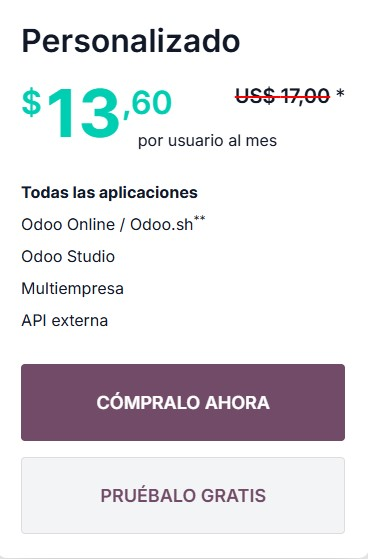
\includegraphics[width=0.3\textwidth]{assets/oddopricing.JPG}
  \caption{Costo mensual por usuario de un ERP popular}
  \label{fig:oddopricing}
\end{figure}

Además, los procesos productivos de la empresa presentan características específicas que no son plenamente compatibles con los flujos estándar de un ERP tradicional.
Esto genera un sobredimensionamiento del sistema, con funcionalidades innecesarias que no sólo complican su uso, sino que también incrementan los costos de implementación, capacitación y mantenimiento.

Por otro lado, la empresa no requiere la gama completa de funciones que un ERP ofrece. Su necesidad se centra en las actividades de planeación de materiales y recursos (MRP) propias de su modelo de producción, como la gestión de inventarios, la programación de pedidos y el control de recursos para cumplir con los tiempos de entrega.
Sin embargo, las soluciones actuales no ofrecen un equilibrio adecuado entre simplicidad, accesibilidad y personalización, dejando un vacío importante en su capacidad operativa.

Esto plantea la necesidad de desarrollar una solución de software específica que no solo atienda la problemática original del control de inventarios y cálculo continuo de costos de producción, sino que también sea accesible para usuarios sin formación técnica avanzada y optimice los procesos productivos sin introducir complejidad innecesaria.
Un sistema diseñado a medida puede resolver estas problemáticas al enfocarse exclusivamente en las funcionalidades necesarias y al ofrecer una interfaz amigable y adecuada para el perfil de los usuarios finales.

% \section{Objetivos}

\subsection{Objetivo General}

Desarrollar un sistema integrado de gestión, control y planificación de actividades de producción para la empresa de prefabricados ArenA,
que sea sencillo de usar, responda a los flujos de trabajo específicos de la empresa y contemple ciertos aspectos propios de un MRP II,
como el manejo de inventarios de producción, cálculo de costos de fabricación, registro de compras, ventas, clientes y proveedores; registro de máquinas y actividades de mantenimiento; registro y gestión de recursos humanos; y despliegue de reportes útiles para la toma de decisiones.

\subsection{Objetivos Específicos}

La concreción de este objetivo involucrará de forma necesaria la realización de
las actividades siguientes como objetivos específicos:

\begin{itemize}
    \item Crear una comunidad de proyectos de código abierto alrededor de éste.
\end{itemize}
% \section{Justificación}
La solución propuesta tiene 3 pilares importantes que la componen y muestran relevancia cada una por su cuenta:

\begin{itemize}
    \item La figura del paquete de software reutilizable.
    \item La figura del trámite en instancias gubernamentales y su modernización.
    \item El desarrollo de software libre.
\end{itemize}

De acuerdo a esto podemos ver la importancia de esta solución en distintos ámbitos:

\subsection{Tecnológico}
La creación de un paquete de software reutilizable para la creación y
seguimiento de trámites ayuda en el proceso de digitalización de uno de los
procedimientos más comunes en el ámbito público, brinda a los gobiernos la
posibilidad de aprovechar de mejor manera los datos resultantes de un trámite y
dan a la población herramientas que hacen más fáciles sus vidas.

Al usar máquinas de estados finitas logramos el aprovechamiento del conocimiento
en sistemas secuenciales digitales dentro del ámbito de sistemas de software
para lograr una abstracción del trámite.

El paquete no sólo facilitará la implementación de sistemas de software con
módulos de trámites, sino que de forma más directa simplificará la tarea de los
desarrolladores, siendo una pieza tecnológica dentro de proyectos más amplios.

\subsection{Económico}
El software reutilizable de código abierto suele ser aprovechado hoy en día con el objetivo de
disminuir costos en la producción de sistemas gracias a su naturaleza de
comunidad y lo demandado de su funcionalidad.

De no existir el software reutilizable se deben invertir recursos para cada
proyecto que requiera la misma funcionalidad. Recursos que, de usar un paquete
de software, podrían conservarse, siendo que una parte del desarrollo ya estaría
implementada. Existen excepciones a este caso en proyectos con necesidades muy
específicas, pero en la mayoría de proyectos, una librería o \textit{framework} bien
implementado son esenciales para disminuir costos de producción.

\subsection{Académico}
Los proyectos de software libre a nivel regional y a nivel universidad son
realmente escasos y al momento de redacción de este documento se desconoce de
algún caso de éxito en la carrera de Ingeniería Electrónica de la UMSA.

Es por eso que este proyecto busca ser un punto de partida hacia la realización
de más proyectos del mismo tipo, es decir, de software libre reutilizable. Todo
esto a partir de esta travesía que a modo de ejemplo busca inspirar a más
estudiantes de la carrera.

\subsection{Político}
La realización de este proyecto no sólo se alinea con la necesidad de los
distintos gobiernos del mundo de digitalizar sus procesos administrativos - como
se puede constatar en Bolivia por el decreto xxx donde se solicita a las
distintas instituciones gubernamentales la realización de planes hacia un
gobierno electrónico -, sino además apunta a la preferencia que los gobiernos
tienen por el software libre, como se describe en el artículo xx de la ley xx.

\subsection{Social}
Los trámites son un dolor de cabeza para gran parte de la sociedad. Los
gobiernos hacen el intento por digitalizar los mismos y así aliviar a la
población, pero la existencia de herramientas reutilizables pueden acelerar
drásticamente este proceso. Se espera que más y más trámites sean digitalizados
en tanto más fácil sea hacerlo. De esta manera los distintos actores de la
sociedad podrán aprovechar las bondades de las tecnologías de la información.

La digitalización de trámites, que sería facilitada por este proyecto, mejora
además los mecanismos por los cuales la sociedad participa del gobierno. Impulsa
la apertura de la información de los gobiernos hacia la gente y se adecúa a las
nuevas necesidades de las personas.
% \section{Alcances y Limitaciones}

De acuerdo a los objetivos planteados es menester delinear el campo de acción del proyecto.

\subsection{Alcances}

\begin{itemize}
    \item Se desarrollará un paquete de software en su primera versión con funcionalidades para facilitar la creación y seguimiento de trámites.
    \item Tunkunia será distribuido mediante al menos un repositorio remoto de versionado como \textit{GitHub}.
    \item El producto además será publicado en algún repositorio de paquetes de software coherente con la tecnología que use.
    \item Se usará una licencia de software libre que permita el uso de esta idea sin restricciones, pero mencionando al autor.
    \item El proyecto contará con la implementación de una documentación en línea para facilitar el uso de Tunkunia.
    \item Se demostrará el uso del paquete en una implementación de un \textit{fork} del sistema SIAI.
    \item Se usarán buenas prácticas de programación para lograr código legible y sobre el cual sea sencillo colaborar.
    \item Los lineamientos, fruto de la creación conceptual de este software serán creados con la ayuda de herramientas para desarrolladores como un CLI.
    \item Se recibirá al menos un \textit{pull request} en el repositorio para demostrar las bondades del software libre y se atenderá al menos un \textit{issue} reportado.
    \item Se adoptarán medidas de \textit{testing} para entregar un mejor código.

\end{itemize}

\subsection{Limitaciones}

\begin{itemize}
    \item El desarrollo no será realizado desde cero y de forma completa, sino que siguiendo los mismos lineamientos sobre los cuales se piensa este proyecto de software, se usarán herramientas de software libre como ladrillos de construcción para éste. Esto puede ser considerado un alcance de acuerdo a cómo se lo vea.
    \item La versión 1 será funcional, pero no se garantiza que esté libre de bugs, lo cual es natural en muchos desarrollos de software a pesar de la aplicación de las mejores prácticas y el testing.
    \item El sistema, si bien podría ser utilizado por un amplio abánico de aplicaciones, en su versión 1, que es la que atañe a este documento, se centrará unicamente en los trámites públicos más comunes y sin cubrir necesariamente las necesidades de cualquier trámite que pueda existir. Se deben tomar como marco los trámites realizados en el sistema SIAI, que es el caso de estudio sobre el cual se desarrollará Tunkunia.
    \item Si bien este proyecto puede ser aplicado en distintos entornos de manera conceptual, debe quedar claro que la implementación práctica de cualquier paquete de software suele estar acotada a ciertas tecnologías. En el caso presente esta tecnología será \textit{Laravel} por su presencia en el sistema SIAI y por su crecimiento reciente en popularidad.
\end{itemize}
% \section{Descripción de la Solución Propuesta}
Dada la problemática expuesta en la sección \ref{problem_statement}, en esta sección
se describe una primera aproximación a su solución de forma detallada.

Se propone desarrollar una herramienta a medida diseñada para satisfacer las necesidades específicas de la empresa de prefabricados ArenA en sus procesos productivos,
optimizando la gestión de inventarios, el cálculo de costos de fabricación y la planificación de la producción.

Este sistema implementará varias características comúnmente encontradas en un MRP (Material Requirements Planning), e incorporará también ciertas otras características existentes en un 
MRP II (Manufacturing Resource Planning) para cubrir procesos clave del negocio de manera sencilla y eficiente, en particular en el área de manufactura. 
Nótese, sin embargo, que ante el nivel de personalización y la no tan estricta definición de un MRP II, no se pretende ser una copia exacta de este tipo de sistemas, teniendo identificadas como necesarias de forma amplia las siguientes características.

\subsection{Características Principales}

\begin{enumerate}
  \item Gestión de Inventarios y Cálculo de Costos
        \begin{itemize}
          \item Registro y control de inventarios de materias primas, productos en proceso y productos terminados.
          \item Cálculo automatizado de costos de fabricación, basado en el consumo de materiales y las actividades registradas en el proceso de producción.
          \item Alertas automáticas ante niveles bajos de materias primas o cuando los almacenes de productos terminados estén al máximo de su capacidad.
          \item Registro de almacenes atómicos para un análisis detallado y fácil ubicación de artículos 
        \end{itemize}
        
  \item Abstracción de actividades principales del negocio
        \begin{itemize}
          \item Adaptación de actividades de compra, venta y fabricación en las distintas etapas productivas
          \item Creación de actividades personalizadas para nuevos procesos de fabricación
        \end{itemize}

  \item Registro de Compras y Ventas
        \begin{itemize}
          \item Registro detallado de compras de materias primas, asociado con información de proveedores.
          \item Control de envíos de productos terminados hacia las áreas de ventas, garantizando una integración fluida entre la producción y la comercialización.
        \end{itemize}

  \item Información sobre Proveedores y Compradores
        \begin{itemize}
          \item Base de datos para almacenar información clave sobre proveedores, como contactos, condiciones de entrega y tiempos de suministro.
          \item Base de datos de compradores con información de contacto y relación histórica con compras realizadas.
        \end{itemize}

  \item Generación de Reportes y Predicciones
        \begin{itemize}
          \item Reportes detallados sobre consumo de materias primas, costos de producción, inventarios y envíos.
          \item Reportes fáciles de emplear por el área contable en formato Excel.
          \item Predicciones automáticas sobre la demanda en base a datos históricos 
        \end{itemize}

  \item Interfaz Adaptada al Modelo de Negocio
        \begin{itemize}
          \item La interfaz estará diseñada para que los usuarios puedan registrar actividades específicas del modelo de negocio, sin necesidad de comprender conceptos técnicos contables como el de inventarios. Por ejemplo, al presionar un botón de "Quema en el horno de ladrillos", el sistema actualizará automáticamente los inventarios correspondientes (materias primas consumidas, productos en proceso y productos terminados).
        \end{itemize}
  \item Restful API para posibilitar la interoperabilidad
        \begin{itemize}
          \item Endpoints para registrar cambios en el inventario de manera automatizada desde sistemas de monitoreo o adquisición de datos como ser los sistemas SCADA (Que tengan habilitada la función de conexiones http)
          \item Endpoints para obtención de información relevante en el sitio principal de la empresa o en sus aplicativos de cálculo de materiales orientados al cliente
        \end{itemize}
  \item Registro de Maquinaria, Materiales y Mano de Obra
        \begin{itemize}
          \item Registro de máquinas con su consumo energético y otros datos relevantes como su estado de operación.
          \item Registro de materiales y su estado, para alertar sobre posibles necesidades de renovación.
          \item Registro de obreros con sus habilidades y competencias para optimizar la asignación a tareas específicas.
        \end{itemize}
\end{enumerate}

\subsection{Beneficios del Sistema}

Algunos de los beneficios que se conseguirán con este sistema son:

\begin{itemize}
\item Accesibilidad y Simplicidad: Una interfaz amigable y adaptada al flujo de trabajo real de la empresa, diseñada para usuarios sin formación técnica avanzada.

\item Automatización y Eficiencia: Reducción de errores y tareas manuales al integrar y automatizar procesos de inventario.

\item Asistencia en el cálculo de costos de producción basado en datos objetivos e históricos, respondiendo a cambios en el mercado de forma inmediata.

\item Toma de Decisiones Basada en Datos: Reportes y predicciones precisos que respaldan la planificación y optimización de recursos.

\item Personalización: Adecuación específica a las características y necesidades únicas del negocio, evitando la complejidad innecesaria de soluciones genéricas.
\end{itemize}

Con este sistema, la empresa podrá gestionar de manera eficiente sus inventarios y procesos de producción, alineándose con sus objetivos operativos y asegurando un uso óptimo de sus recursos.

% Arquitectura propuesta
% \section{Presupuesto Tentativo}
% \section{Temario} \label{syllabus}

\begin{figure}[!thpb]
    \centering
    \includegraphics[width=0.7\textwidth]{assets/proceso_pressman_white}
    \caption{Proceso del Software - Pressman}
    \label{fig:proceso_pressman}
\end{figure}

Para el temario del documento final de proyecto se considerará una estructura que describa bien la naturaleza del proyecto y que además se adecúe a este que, después de todo, será un producto de software.

De acuerdo a la ingeniería de software, el software tiene un ciclo de vida o un \say{proceso del software}, el cual se modela de acuerdo a la metodología de desarrollo sobre la cual se realice. Sin embargo, varios autores concuerdan en que existen ciertas etapas estructurales ajenas a cualquier metodología. Según \textit{Pressman} \cite[13]{pressmanSoftwareEngineeringPractitioner2010}, estas etapas serían las indicadas en la figura \ref{fig:proceso_pressman}.

Por su lado, \textit{Sommerville} las simplifica en las 4 etapas mostradas en la figura \ref{fig:proceso_sommerville}.

\begin{figure}[!thpb]
    \centering
    \includegraphics[width=0.7\textwidth]{assets/proceso_sommerville_white.pdf}
    \caption{Proceso del Software - Sommerville}
    \label{fig:proceso_sommerville}
\end{figure}

El temario del documento final del proyecto obedecerá entonces a esta definiciones del proceso de software para no depender estrictamente de la metodología usada.

Nótese, sin embargo, que este temario es tentativo, lo cual quiere decir que pueden surgir cambios durante la realización del proyecto.

\begin{tcolorbox}[breakable]

    \subsection*{\Large{Índice}}
    \begin{syllabus}
        \item[0.] Apartados Preliminares
        \begin{itemize}
            \item Presentación
            \item Agradecimientos
            \item Resumen
            \item Índice
            \item Glosario
        \end{itemize}
    \end{syllabus}

    \begin{syllabus}
        \item \textbf{Generalidades del proyecto:}
        \begin{syllabus}
            \item \textbf{Introducción:} Describirá los antecedentes del proyecto, así como la problemática que se ha identificado, para la cual se plantea una solución a través del objetivo. De igual modo se hará referencia a la justificación del proyecto y los alcances y límites que se plantearon durante su gestación.
            \item \textbf{Marco Referencial:} Se proporciona el contexto general en el cual se sitúa el proyecto. Se describen temas relevantes al tópico principal y que buscan delimitarlo en varios aspectos que pueden ser históricos, geográficos, sociales, políticos, económicos, tecnológicos, etc.
            \item \textbf{Marco Teórico:} Se proporcionan las bases teóricas sobre las cuales se fundamenta el proyecto. se presentarán todos los conceptos, definiciones, técnicas y/o procedimientos que se han de tomar en cuenta para el desarrollo del proyecto y para su correcta comprensión.
        \end{syllabus}
        \item \textbf{Proceso del Software:} Como se explica al inicio de la sección \ref{syllabus}, esta parte del temario reflejará el ciclo de vida común del software. El orden no refleja el orden que se adopte realmente, el cual no será de tipo cascada, sino iterativo, pero como bloques fundamentales del proceso del software, tendrán la información relevante a cada etapa o cada esfuerzo realizado dentro de cada etapa.
        \begin{syllabus}
            \item Especificación de requerimientos de software \cite[104]{pressmanSoftwareEngineeringPractitioner2010}
            \item Modelado y Diseño
            \item Desarrollo y Construcción
            \item Pruebas y Validaciones (Tests)
            \item Despliegue
        \end{syllabus}
        \item \textbf{Integración en el SIAI:} El paquete ya desplegado se integrará en un \textit{fork} del SIAI. En este apartado se hará una bitácora del proceso y se expondrán los resultados del mismo.
        \item \textbf{Resultados y Conclusiones:} El resultado general del proyecto y algunas recomendaciones para seguir trabajando en él, siendo especialmente importante considerando la naturaleza \textit{open source} y colaborativa del paquete a desarrollar. Se deben dar algunas ideas para seguir desarrollando las siguientes versiones del software.
    \end{syllabus}

    \begin{itemize}
        \item Bibliografía y Referencias
        \item Anexos
    \end{itemize}
\end{tcolorbox}
% \section{Cronograma}

\begin{figure}[!ht]
    \centering
    \includegraphics[width=0.7\textwidth]{assets/rupphases}
    \caption{Fases del Proceso Unificado y los esfuerzos de cada actividad en las mismas}
    \label{fig:rupphases}
\end{figure}

El cronograma de trabajo (figura \ref{fig:gantt}) estará fuertemente influenciado por las fases de la metodología \textit{RUP (Rational Unified Process)}, la cual cuenta con 4 fases y 6 actividades principales que se realizan de forma iterativa en cada una de estas fases. La figura \textit{\ref{fig:rupphases}} muestra cuánto de cada actividad se debe realizar en cada etapa y permite entender el cronograma presentado.

\begin{figure}
    
\begin{ganttchart}[
        vgrid,
        hgrid,
        x unit=\textwidth/33,
        bar label node/.append style={text width=2.5cm, align=right}
    ]{1}{25}
    % TITLE
    \gantttitle{Tunkunia - 25 Semanas}{25} \\
    \gantttitlelist{1,...,25}{1} \\

    % Tareas generales
    \ganttbar{Investigación}{1}{2} \\
    \ganttbar[name=mem0]{Redacción Memoria}{4}{7}
    \ganttbar[name=mem1]{Redacción Memoria}{16}{18}
    \ganttbar[name=mem2]{Redacción Memoria}{22}{25} \\
    \ganttlinkedmilestone{Presentación}{25} \\

    % Tareas del desarrollo en sí mismo
    \ganttgroup[name=rup]{Iteraciones RUP}{3}{18} \\
    \ganttbar[name=in]{Inception}{3}{4} \\
    \ganttlinkedbar{Elaboration}{5}{7} \\
    \ganttlinkedbar[name=const]{Construction}{8}{15} \\
    \ganttlinkedbar{Transition}{16}{17} \\
    \ganttlinkedbar[name=doc]{Documentación}{18}{18} \\

    % Aplicación y posteriores
    \ganttgroup[name=use]{Aplicación}{19}{22} \\
    \ganttbar[name=fork]{Fork del SIAI}{19}{19} \\
    \ganttlinkedbar{Integración}{20}{21} \\
    \ganttlinkedbar{Pruebas}{22}{22}

    % Milestones
    %\ganttlink{elem0}{in}
    \ganttlink{doc}{fork}
    %\ganttlink{const}{mem}
\end{ganttchart}
    \caption{Diagrama de Gantt del proyecto}
    \label{fig:gantt}
\end{figure}
Se debe notar que la redacción de la memoria se realizará de forma paralela al desarrollo del proyecto, al igual que el proceso de Investigación. Sin embargo, en el diagrama de Gantt se muestran las semanas en las que estas dos actividades tomarán prioridad.
\clearpage
\printbibliography
\addcontentsline{toc}{section}{Bibliografía y Referencias}
\end{document}